

Há muitos aspectos na construção de um sistema de visão confiável, este deve ser compatível com um robô de ação rápida, sem sobrecarregar nenhum dos processos de visão. 
Esse capítulo começa na seção ~\ref{exp:robo} fazendo uma breve introdução ao hardware do robô que foi utilizado para execução dos experimentos, o mesmo continua apresentando experimentos para identificação da bola laranja seção ~\ref{exp:bollar} e da bola branca~\ref{exp:bolbra}, assim como o cálculo de suas distâncias ao robô na seção ~\ref{exp:balldist}. Os experimentos da detecção de robôs se iniciam com a seção ~\ref{exp:HOG-SVM} onde o algoritmo  HOG-SVM foi comparado com o detector de pedestres clássico com imagens de humanos e com poucas imagens de treinamento para robôs. Na seção ~\ref{exp:HAAR-Boosting} o detector de robôs foi implementado com o uso do HAAR-Adaboost. Na seção ~\ref{exp:comp}, os algoritmos HOG-SVM e HAAR-Adaboost são postos em perspectiva, ambos com os mesmos parâmetros e quantidade de imagens, de modo que algumas conclusões podem ser tomadas apresentando os resultados de cada experimento em sua respectiva seção.

\section{O robô}
\label{exp:robo}
Quatro robôs humanoides autônomos foram desenvolvidos para atuar na liga KidSize da RoboCup. Para os experimentos do presente, o robô utilizado foi o B2, robô baseado no DARwIn-OP \cite{Darwin}, veja figura ~\ref{Fig:Darwin} desenvolvido no Centro Universitário da FEI. O robô DARwIn-OP tem sua plataforma aberta, que foi criada e desenvolvida pela fabricante coreana de robôs ROBOTIS em colaboração com a Virginia Tech, a Universidade de Purdue e a Universidade da Pennsylvania. O DARwIn-OP têm vinte graus de liberdade sendo cada um desses graus controlado por um servo-mecanismo DYNAMIXEL MX-28T.

Duas grandes modificações foram feitas: A primeira foi a extinção do microcontrolador ARM 32-bit Cortex-M3, responsável pelo controle de baixo nível dos servos mecanismos, isso implica que os pacotes enviados para os servos do pan-tilt precisam ser enviados da porta USB do computador através de um conversor RS485 para os servos, a segunda foi a instalação da câmera modelo c920, full hd e 78 graus de campo de visão, da Logitech. 

O peito do robô teve que ser redesenhado e reimpresso em uma impressora 3D, de modo que, seu espaço foi aumentado para que fosse possível a substituição do mini-computador com processador Intel Atom Z530 1.6GHz por um Intel NUC Core I5 com 2.5GHz, 4Gb de RAM e placa de vídeo HD Graphics 4000 com capacidades de trabalhar com resoluções de 4K.

O sistema operacional usado foi o linux Ubuntu 12.04. Usando a posição pan-tilt proveniente da biblioteca fornecida pela Dynamixel, fornecedora dos servo-mecanismos. Vários testes foram executados com os diversos objetos presentes no campo, sob diversas condições de luz. Os algoritmos foram desenvolvidos em C++, em conjunto com a biblioteca open source \citeonline{OpenCV}.

\begin{figure}[!t]
\centering \caption{O Robô Darwin Modificado.}
\includegraphics[width=3.5in]{Imagens/resized-darwin.jpg}
\DeclareGraphicsExtensions.
\caption*{Fonte: Autor}
\label{Fig:Darwin}
\end{figure}


\section{Experimento - Encontrando uma bola laranja usando segmentação e transformada de Hough para círculos}
\label{exp:bollar}
Esse experimento foi implementado conforme o algoritimo ~\ref{lst:algBall} e foi testado em diversas situações de variação de luz e oclusão.

Os parâmetros do HSV podem assumir valores de 0 à 359 para a matiz, de 0 à 255 para a saturação e para a intensidade. Como parte dos requisitos de calibração da cor referente à bola, um algoritmo utilizando barras de rolagem (trackbars) foi implementado de forma que era possível alterar os parâmetros da segmentação apresentando-a em tempo real. Alterando esses três parâmetros foi possível visualizar quando a bola se tornava discrepante do fundo. Os valores encontrados variaram de 0 a 35 graus para a matiz, de 0 a 200 para a saturação e 0 a 180 para a intensidade dependendo da iluminação do local.

Dessa forma, para a LUT a matiz foi discretizada em 7 passos de 5 graus cada, a saturação em 10 passos e a intensidade em 10. Isso reduz o tempo de segmentação, pois o algoritmo tem que percorrer menos estados para efetuar a segmentação.

O pré-processamento é um dos fatores cruciais para se utilizar os círculos de Hough com alguma precisão. Ao testar diversos valores para o limiar do acumulador, este parece ser um parâmetro chave. Basicamente quanto maior for esse limiar menos círculos são detectados, mesmo assim esses círculos têm uma probabilidade maior de serem detectados corretamente \cite{Davies}. É possível fazer uma busca de parâmetros binária até que um certo critério seja atingido, no caso apenas um círculo. O valor definido, após algumas tentativas, ficou estabelecido em 50. 

Para os círculos de Hough, o tamanho máximo do círculo a ser detectado foi limitado à 30 pixels de diâmetro, essa escolha visa reduzir os falsos positivos e ruídos, mas também possui o revés de reduzir o alcance de detecção da bola, que nesse caso ficou limitado a 3 metros. De forma análoga, o tamanho máximo de detecção ficou definido como sendo a largura da tela dividido por 2, visto que a bola, estando no chão, nunca terá um tamanho maior que esse.

Outra forma de reduzir os falsos positivos foi utilizar a informação temporal da câmera e armazenar na forma de média móvel (Ver referência de séries temporais no “ANEXO A”, trecho do trabalho de \citeonline{Lopes}) a posição e raio atual da bola. As posições cartesianas da bola dos últimos 10 quadros são armazenados e têm sua média aritmética calculada em forma de fila, assim uma falsa detecção que não representa uma bola tem sua influência reduzida na posição real da bola. 

Durante os experimentos, enquanto a bola esteve no campo de visão da câmera, esse algoritmo de rastreamento bola provou ser muito confiável mesmo quando um borramento é causado pelo movimento da bola. Este algoritmo foi amplamente testado para oclusão parcial (Veja figura ~\ref{fig:occluded}) e robustez em diferentes condições de iluminação, incluindo a luz direta do sol e sombras (ver Figura ~\ref{Fig:SegBall}).

Na medida que o tamanho da bola, em pixels, é extremamente importante para calcular a distância verdadeira bola, a oclusão é um problema difícil que tem de ser resolvido. Os testes mostrados na figura ~\ref{fig:occluded} demonstram o algoritmo estimando o raio da bola, mesmo quando a maior parte da esfera está oculta. Se o formato for prejudicado por qualquer motivo a distância real da bola também o será. 

Foi feito um teste com a bola, no qual o algoritmo proposto foi complementado com o algoritmo de condensação, ver figura ~\ref{Fig:CondBall}, citado no capítulo de trabalhos correlatos. Nesse teste, enquanto a bola se encontrava à uma distância menor do que 2 metros, o algoritmo de rastreamento executava os círculos de Hough, assim que a mesma se distanciava além desse limite, o algoritmo mudava para o de condensação onde 1.500 partículas foram utilizadas como uma forma de identificar probabilisticamente a posição da bola. Essa quantidade de partículas foi definida após contabilizar a área, em pixels, referente à bola quando essa se encontrava a 6 metros do robô, na resolução full-hd, onde possuía o raio de 22 pixels.

Apesar dos resultados animadores, onde foi possível estimar a posição da bola a mais de 6 metros, ver tabela ~\ref{Tab:ResBola}, não foi possível adequar essas duas técnicas juntamente com o restante do sistema de visão. Esse algoritmo, de forma individual, manteve a taxa de quadros por segundo de 28, porém, ao incluir os outros algoritmos, o mesmo apresentou problemas de lentidão e acabou cessando de funcionar após apenas alguns segundos, indicando que possa ter havido uma exigência muito grande do processador, fato comprovado pelo monitor de sistema do Ubuntu.

\begin{figure}[!ht]
\centering \caption{O robô Darwin seguindo uma bola parcialmente oculta pelo seu braço.}%

\parbox{2.5in}{\includegraphics[width=2.5in]{Imagens/resized-3.png}\center{\fontsize{10pt}{10pt}\selectfont (a)}} 
\qquad 
\begin{minipage}{2.5in}%
\includegraphics[width=2.5in]{Imagens/resized-1.png}
\center{\fontsize{10pt}{10pt}\selectfont (c)}
\end{minipage}
\vspace*{3mm}

\parbox{2.5in}{\includegraphics[width=2.5in]{Imagens/resized-4.png}\center{\fontsize{10pt}{10pt}\selectfont (b)}} 
\qquad
\begin{minipage}{2.5in}%
\includegraphics[width=2.5in]{Imagens/resized-2.png}\center{\fontsize{10pt}{10pt}\selectfont (d)}
\end{minipage}%

\caption*{Fonte: Autor}%
\label{fig:occluded}%
\end{figure}


\begin{figure}[!ht]
\centering \caption{Robô Milton seguindo a bola com a influência da luz do sol e sombras.}
\includegraphics[width=7cm]{Imagens/Sun_Ball1.jpeg}
\includegraphics[width=7cm]{Imagens/Sun_Ball2.jpeg}
\DeclareGraphicsExtensions.
\caption*{Fonte: Autor}
\label{Fig:SegBall}
\end{figure}


\begin{table}[ht!]
    \caption{Resultados dos algoritmos para reconhecimento da Bola} \label{tbl:Bola}
    \centering
    \begin{tabular}{|c|c|c|c|}
    \hline 
    Descrição & Círculos de Hough & Condensação\\ 
    \hline 
    Alcance da detecção (Centímetros) & 300 & 600\\ 
    \hline 
    Quadros por segundo & 30 & 28\\ 
    \hline 
    \end{tabular}
    \caption*{Fonte: Autor}
    \label{Tab:ResBola}
\end{table}

\begin{figure}[!ht]
\centering \caption{B1 utilizando a condensação para identificar probabilisticamente e qualitativamente a posição da bola laranja no quadro.}
\includegraphics[width=7cm]{Imagens/BolaLar/BL1.jpg}
\includegraphics[width=7cm]{Imagens/BolaLar/BL2.jpg}
\DeclareGraphicsExtensions.
\caption*{Fonte: Autor}
\label{Fig:CondBall}
\end{figure}




\section{Experimento - Encontrando uma bola branca usando características HAAR}
\label{exp:bolbra}
A liga humanoide da RoboCup, vislumbrando a meta de 2050, vem fazendo diversas mudanças no campo e em seus objetos, incluindo a bola. A principal alteração efetuada foi a troca de sua cor predominantemente alaranjada, passando a ser no mínimo 80 por cento branca. A mudança das características da bola fez com fosse necessário uma mudança de paradigma para efetuar sua detecção. A segmentação por cores passou a apresentar diversos falsos positivos, basicamente devido ao brilho causado pelo reflexo branco da luz em diversos objetos que não representavam a bola. Assim, tendo como meta sanar esse revés, foi implementado um algoritmo utilizado as características de HAAR como descritor.

Um conjunto de imagens positivas e negativas foram coletadas na resolução full-hd (1920x1080 pixels). Aqui um conjunto de imagens negativas foi adquirida visando a diversidade contendo imagens de locais diversos como prédios, campos de futebol, multidões e ruas, sem que a bola estivesse envolvida.

As imagens positivas foram reunidas posicionando a bola em diferentes distâncias da câmera do robô e em diversas posições no campo de futebol.
As imagens estão á disposição no endereço (https://www.copy.com/id-568856/imagens). O total de imagens positivas colhidas foi de 2135 imagens, já as negativas somaram 1192 imagens. 

A janela mínima de detecção foi definida com 20x20 pixels, ou seja, o menor objeto (bola) a ser detectado terá essa dimensão. Essa janela foi escolhida visto que ela representa uma bola a 8 metros de distância. Essa distância é suficientemente pequena para que o robô estando em um lado do campo possa reconhecê-la do outro lado e, de forma oposta, não tão pequena que possam ser detectados falsos positivos. Durante o treinamento o número máximo de estágios foi determinado como sendo de 20 estágios, a taxa de acerto mínima foi configurada em 0.999, o parâmetro \(N_{\text{AmostrasPositivas}}\) após cálculo utilizando as equações ~\ref{eq1} e ~\ref{eq2} ficou fixada em 920, finalmente, a janela de amostragem foi de 100x100 pixels. O classificador utilizado foi k vizinhos mais próximos (K-nearest neighbors) com valor de k = 11. Outros valores menores foram escolhas claramente ruins, já que geraram diversos falsos positivos. Bons resultados apareceram com o valor de k=9 mas, também geraram diversos falso positivos em diversas circunstâncias. A classificação ficou prejudicada com valores maiores valores de k.

Todos os objetos, foram selecionados manualmente usando uma caixa delimitadora retangular a partir das imagens positivas. O utilitário Criar amostras da biblioteca opencv \cite{OpenCV} foi usado para criar amostras de treinamento de cada imagem, enquanto alimentava um vetor.

Cada estágio do classificador foi dividido em dois nós, de modo que o resultado do classificador para cada nó foi armazenado em um arquivo xml.

No experimento apresentado na figura ~\ref{fig:BolaHaar}, duas bolas brancas idênticas estão posicionadas em posições diferentes (5 e 7 metros) em um campo de futebol de grama sintética sobrecarregado de objetos e pessoas se movendo. 

\begin{figure}[!ht]
    \centering \caption{Rastreamento da bola usando características HAAR em um campo de futebol sobrecarregado de objetos, pessoas e regiões não pertencentes ao jogo.}
    \subfloat[]{{\includegraphics[width=7cm]{Imagens/Bola/B04.png} }}%c
    \qquad
    \subfloat[]{{\includegraphics[width=7cm]{Imagens/Bola/B05.png} }}%d
    \qquad
    \subfloat[]{{\includegraphics[width=7cm]{Imagens/Bola/B12.png} }}%j
    \qquad
    \subfloat[]{{\includegraphics[width=7cm]{Imagens/Bola/B37.png} }}%u

    \caption*{Fonte: Autor}
    \label{fig:BolaHaar}
\end{figure}

Na figura ~\ref{fig:RocBolaHaar}, a curva ROC demonstra os resultados da detecção.


\begin{figure}[!ht]
    \centering 
    \includegraphics[width=14cm]{Imagens/Curva_ROC_Bola.png}
    \caption[Curva ROC para detecção da bola usando características HAAR.]{Fonte: Autor}
    \label{fig:RocBolaHaar}
\end{figure}

\section{Experimento - Determinação da distância da bola ao robô}
\label{exp:balldist}
Os cálculos das distâncias da bola e do robô até outros robôs, foram determinados de forma experimental, tabelando a distância em centímetros e a área dos objetos em pixels, encontrando por meio de regressão a função que representasse essa relação, considerando, é claro, a resolução da captura. 

O principal objetivo da média móvel simples é fornecer o valor médio do raio da bola e sua posição em pixels dentro de um determinado período, no caso, os últimos 10 quadros da captura de video. Médias Móveis eliminam grandes oscilações nos valores, filtrando somente a posição principal. Quanto maior o período utilizado na Média Móvel maior é o grau de filtragem. Assim, para cada valor incluído no cálculo da média, o valor mais antigo é excluído. Na média móvel simples (SMA), cada dado utilizado no cálculo da média terá o mesmo peso. 

\begin{equation} 
\label{eq:MM}
	MRB = \frac {[R(q) + R(q-1) + R(q-2) + . . . + R(q-9)]}  {10}
\end{equation}

MRB é a média móvel do raio da bola e R é o raio da bola ambos em pixels, já q se refere ao índice do quadro atual da captura da câmera. Tabelando os raios médios da bola e sua distância real em centímetros, é possível por meio de regressão estimar uma função que representa os dados. O experimento foi realizado posicionando a bola no pé do robô e afastado-a do pé do robô com incrementos de 5 centímetros, a cada incremento foi coletado o diâmetro médio da bola em pixels, após coletar 30 pontos o gráfico na figura ~\ref{Fig:DistBall} foi plotado. 

\begin{figure}[!t]
\centering \caption{Função relacionando pixels com distância de uma bola de tamanho conhecido.}
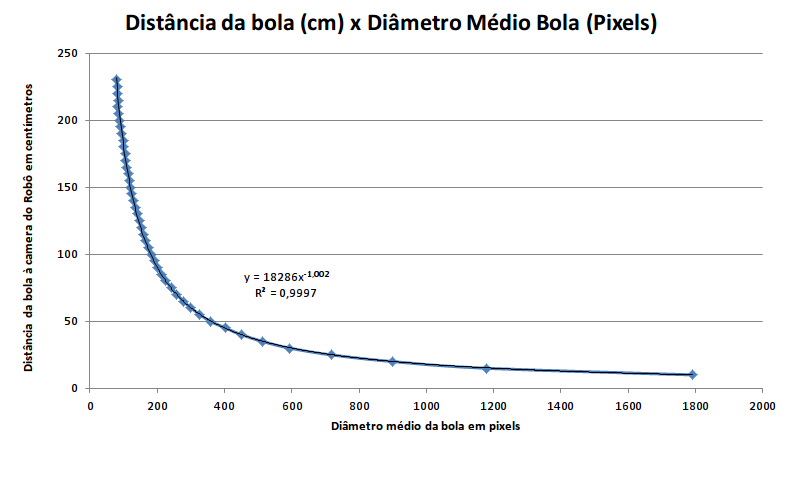
\includegraphics[width=15cm]{Imagens/Dist.png}
\DeclareGraphicsExtensions.
\caption*{Fonte: Autor.}
\label{Fig:DistBall}
\end{figure}

A função que relaciona o tamanho da bola em pixels com a distância da bola em centímetros foi extraída por meio de uma regressão não-linear exponencial, disponível no software Ms-Excel \cite{MS}, para a resolução de 1920x1080 pixels, bola de tamanho fixo e conhecido de 13 centímetros, onde \(D_{\text{Bola}}\) é a distância da bola ao robô em centímetros, e MRB é a média móvel do raio da bola em pixels.

O coeficiente de determinação \(R^2\) deve ser interpretado como a proporção de variação total da variável dependente do eixo Y (Distância da bola em centímetros) que é explicada pela variação da variável independente no eixo X (Tamanho da bola em pixels). Nesse caso pode-se concluir que 99,97 \% das variações de Y são explicadas pela variação de X. Como o gráfico foi plotado em relação ao diâmetro da bola , porém, como ambos os algoritimos fornecem como saída o raio da bola, se faz necessário a conversão do diâmetro em raio dividindo-o por dois.


\begin{equation} 
	%D_{bola} = 3,7.10^{-7} * MRB^4 -7.9e^{-5} * MRB^3 +6.2e^{-3} * MRB^2 -2.2e^{-1} * MRB + 3.7 
	%D_{bola} = 331.59-53.3*log(MRB-50);
	D_{bola} = \frac {\frac {18286} {2}} {MRB} \,\,\,\,\,\,\, \therefore \,\,\,\,\,\,\,\, D_{bola} = \frac {9143} {MRB}\,\,\,\,\,\, (cm)
\end{equation}

É claro que, haverá um erro de medição nessas fórmulas, já que foram calculadas sem oclusão e com o objeto inteiro no campo de visão da câmera, nesse caso, o erro será proporcional à oclusão.

\begin{comment}
\section{Determinação da distância do robô a outros robôs}

Para determinar as distâncias até os robôs adversários, ou até os companheiros de equipe é necessário que se possua todas as dimensões dos robôs da liga. Analisando os TDP's Artigos de descrição dos times de todos os robôs da liga KidSize, foram extraídos as alturas dos mesmos.
A tabela criada possui uma coluna referente ao número do time e uma ou mais colunas referente à altura do robôs de cada time, já que um time pode ter mais de um tipo de robô. 

Antes de se iniciar uma partida, o juiz procura os líderes de cada time para definição de suas respectivas cores. Duas cores são possíveis, o time vermelho tem uma coloração magenta e o time azul tem a cor ciano. Feita a escolha, os times devem revestir seus robôs com as cores definidas. A área mínima desses marcadores é 5x5 centímetros nos braços, pernas e tronco.

A detecção foi feita usando o descritor HAAR conforme parâmetros usados no capitulo ~\ref{HAAR-Boosting}

Somente dentro da janela de detecção do robô é feita uma segmentação da cor previamente escolhida no sistema HSV. Os valores foram discretizados em 20 valores para a matiz, 17 para a saturação e 17 para a intensidade.

Assim, se faz necessário encontrar uma fórmula que relacione a resolução da tela, o tamanho em pixels dos robôs e o tamanho real do robô com a sua distância. \citeonline{Bunden} utilizou uma fórmula que relaciona esses parâmetros para detecção da bola. 

Como o raio da bola e a largura do robô são unidimensionais seria possível utilizar a mesma fórmula, já que a relação .  

\begin{equation}
\label{Eq:Dis1}
d_{w} = \sqrt{ \frac {r_{cm}^2} { tan( \frac {\theta_{x}} {w_{img}} * r_{px}) }  - h_{cam}^2} 
\end{equation}

Onde \(d_{w}\) é a distância em centímetros da bola ao robô, \(r_{cm}\) é o raio real da bola em centímetros, \(\theta_{x}\) é o campo de visão horizontal da câmera em graus, \(w_{img}\) é a largura da imagem em pixels, \(r_{px}\) o raio da bola detectada em pixels e \(h_{cam}\) é a altura da câmera.

Como a janela de detecção é retangular o valor equivalente ao raio da bola foi substituído por metade da largura da janela de detecção \(J_{cm}\) e \(J_{px}\), como mostra a equação ~\ref{Eq:Dist2}.

\begin{equation}
\label{Eq:Dist2}
d_{w} = \sqrt{ \frac {      (\frac {J_{cm}}{2})^2    } { tan( \frac {\theta_{x}} {w_{img}} * \frac{ J_{px}} {2} ) }  - h_{cam}^2} 
\end{equation} 

Aqui, \(J_{cm}\) é a largura real do robô em centímetros extraída dos artigos de descrição dos times e \(J_{px}\) é a largura da janela de detecção em pixels, os outros parâmetros permanecem os mesmos da equação ~\ref{Eq:Dis1}

Duas limitações importantes devem ser observadas nessa abordagem, a primeira decorre da orientação do robô sendo observado, se ele estiver orientado à \(90^0\) com relação ao robô que está visualizando-o, sua largura em pixels será menor ou maior, dependendo do formato do robô e quão simétrico o mesmo é em relação ao plano sagital e/ou frontal, como mostra a figura ~\ref{Fig:Ori}, de forma que o cálculo de sua distância também será prejudicada. 

A função primordial da identificação dos robôs é, em primeira instância, iniciar em tempo hábil uma trajetória que evite uma colisão, em segunda instância e, talvez, mais complicada, envolve um procedimento de passes e jogadas ensaiadas entre robôs. Em ambos os casos uma variação de alguns centímetros no cálculo da distância não terá influência significativa, ao menos no estado atual da competição.

A segunda limitação aparece da própria equação utilizada e sua relação com o algoritmo de detecção. O algoritmo usado por \citeonline{Bunden} usa 3 recursos de checagem para a bola, inclusive um para oclusão, determinando com certa precisão os limites da bola. No caso da detecção dos robôs percebe-se que a detecção não tem limites tão bem definidos, de forma que uma abordagem prática utilizando dados reais dos próprios robôs poderiam apresentar melhores resultados em algum trabalho futuro. 


\pagebreak
\end{comment}
\section{Experimento - Detectando Robôs usando o Descritor HOG com o Classificador SVM}
\label{exp:HOG-SVM}

Sendo o algoritmo mais custoso computacionalmente, o reconhecimento de robôs roda com a resolução de 640x480 pixels e 15 quadros por segundo. O SVM foi treinado com um conjunto de imagens de pedestres humanos, os teste foram executados visando dois tipos de reconhecimento:
\begin{enumerate}
	\item SVM treinado com imagens humanas reconhecendo humanos- (Grupo de controle);
	\item SVM treinado com imagens humanas reconhecendo robôs;
	\item SVM treinado com imagens de robôs reconhecendo robôs.
\end{enumerate}


Para o descritor HOG um descritor padrão de 64x128 pixels foi usado da mesma forma que o artigo original, uma janela de 16x16 pixels, a célula que desliza pela imagem tem 32x32 pixels e um limiar de acerto de 0,5. Para o classificador SVM, o parâmetro de custo C ficou definido em 10 e o parâmetro $\Gamma$ ficou igual a 0.001, ambos escolhidos por uma busca em grade.

Como esperado, o classificador SVM, em conjunto com o descritor HOG, treinado com imagens de pessoas para reconhecimento de robôs é muito menos preciso do que o reconhecimento clássico de imagens de pessoas reconhecendo pessoas, entretanto, mesmo nessas circunstâncias, parece atingir a sua meta. Também foi reunida uma, mesmo que pequena, quantidade de imagens normalizadas contendo robôs, numa tentativa de verificar o quão bom esse algoritmo pode ser. Uma curva ROC foi plotada com as três situações, demonstrado na figura ~\ref{Fig:ROC} e o resultado de um quadro na figura ~\ref{Fig:Miltondet}:

\begin{figure}[!h!t!]
\centering \caption{Curvas ROC. A linha verde mostra o classificador clássico HOG-SVM, usado para reconhecimento de pessoas.
A linha vermelha demonstra o mesmo classificador treinado com pessoas usado para reconhecer robôs e a linha amarela mostra o classificador treinado com 100 imagens de robôs positivas e 100 imagens negativas usado na classificação dos robôs.}
\includegraphics[width=12cm]{Imagens/ROC1.png}
\DeclareGraphicsExtensions.
\caption*{Fonte: Autor \citefloat{Vilao}}
\label{Fig:ROC}
\end{figure}

As curvas ROC sugerem que o classificador treinado com imagens de robôs, mesmo com poucas imagens, parece ser, assintoticamente, melhor que a primeira abordagem usando o conjunto de imagens de pedestres. Nossa expectativa é fazer um classificador de robôs tão bom quanto o que reconhece pedestres. Devido a diversidade de robôs e sendo os seres humanos o nível máximo da forma humanoide, este classificador mostrou uma capacidade de generalização que poderia ser usada para reconhecer uma grande quantidade de robôs humanoides, dada uma quantidade suficiente de imagens de treinamento normalizadas.

\begin{figure}[!h!t!]
\centering \caption{Detecção do robô Milton usando imagens de pessoas como conjunto de treinamento.}
\includegraphics[width=7cm]{Imagens/Milton_Det.jpg}
\DeclareGraphicsExtensions.
\caption*{Fonte: Autor \citefloat{Vilao}}
\label{Fig:Miltondet}
\end{figure} 

É possível ver que a cabeça do robô não foi incluída no retângulo de detecção, talvez, pela falta de imagens normalizadas de boa qualidade ou, talvez, pelo fato da cabeça não estar em conformidade com a cabeça humana.
Como a aquisição de imagens tão específicas com uma mínima qualidade é de certa forma difícil de ser obter, a abordagem "Leave-One-Out" foi utilizada, já que lida bem com poucas amostras de treinamento.


\pagebreak

\section{Experimento - Detectando Robôs usando o Descritor HAAR com o Classificador Boosting}
\label{exp:HAAR-Boosting}
No contexto atual da liga KidSize da RoboCup, outros robôs não têm a necessidade de serem detectados enquanto estiverem a mais de 3 metros de distância, devido a sua velocidade de andar ser bastante reduzida, dessa forma, foi inserida uma limitação com relação à distância do robô a ser detectada.  Assim, a janela mínima de detecção foi definida com 150x150 pixels, ou seja, o menor objeto (robô) a ser detectado terá essa dimensão na imagem. O fato de limitar a janela de detecção mínima tem o principal objetivo de reduzir falsos positivos mas, também de acelerar o processo de detecção, já que menos janelas estarão contidas dentro da imagem. 

Durante o treinamento o número máximo de estágios foi determinado como sendo de 20 estágios, a taxa de acerto mínima foi configurada em 0.999, o parâmetro \(N_{\text{AmostrasPositivas}}\) após cálculo utilizando as equações ~\ref{eq1} e ~\ref{eq2} ficou fixada em 920 para 2135 imagens positivas e 1192 negativas, finalmente, a janela de amostragem foi de 150x150 pixels. O algoritmo foi implementado usando como classificador o k vizinhos mais próximos (K-nearest neighbors) com valor de k = 9. Valores como k=3, k =5 e k=7 foram escolhas claramente ruins, já que geraram diversos falsos positivos. O valor de k=11 teve bons resultados mas, também ignoraram o objeto em diversas circunstâncias. Maiores valores de k não geraram classificação. Mesmo apresentando falsos positivos o Haar conseguiu identificar o robô em diversas situações. Na figura ~\ref{fig:Art} uma sequência de quadros do robô B2 sendo identificado, com o uso do Haar, em um campo de futebol com grama sintética. 

\begin{figure}[!h!t!]
    \centering \caption{Rastreamento do robô B2 usando características HAAR no campo de futebol com grama artificial.}
    \subfloat[]{{\includegraphics[width=4.5cm]{Imagens/Darwin01.png} }}
    \qquad
    \subfloat[]{{\includegraphics[width=4.5cm]{Imagens/Darwin02.png} }}
    \qquad
    \subfloat[]{{\includegraphics[width=4.5cm]{Imagens/Darwin03.png} }}
    \qquad
    \subfloat[]{{\includegraphics[width=4.5cm]{Imagens/Darwin04.png} }}
    \qquad
    \subfloat[]{{\includegraphics[width=4.5cm]{Imagens/Darwin05.png} }}
    \qquad
    \subfloat[]{{\includegraphics[width=4.5cm]{Imagens/Darwin06.png} }}
    \qquad
    \subfloat[]{{\includegraphics[width=4.5cm]{Imagens/Darwin07.png} }}
    \qquad
    \subfloat[]{{\includegraphics[width=4.5cm]{Imagens/Darwin08.png} }}
    \qquad
    \subfloat[]{{\includegraphics[width=4.5cm]{Imagens/Darwin09.png} }}
    \qquad
    \subfloat[]{{\includegraphics[width=4.5cm]{Imagens/Darwin10.png} }}
    \qquad
    \subfloat[]{{\includegraphics[width=4.5cm]{Imagens/Darwin11.png} }}
    \qquad
    \subfloat[]{{\includegraphics[width=4.5cm]{Imagens/Darwin12.png} }}
    \caption*{Fonte: Autor}
    \label{fig:Art}
\end{figure}



\section{Discussão - Comparando os dois descritores e seus classificadores} 
\label{exp:comp}

Diferentemente do experimento apresentado na seção ~\ref{exp:HOG-SVM} nessa seção, as imagens utilizadas para treinamento das técnicas HOG-SVM e HAAR-Adaboost foram as mesmas, ou seja, 2135 imagens positivas e 1192 imagens negativas. Os parâmetros se mativeram os mesmos dos experimentos das seções ~\ref{exp:HOG-SVM} e ~\ref{exp:HAAR-Boosting}.
Duas curvas ROC foram plotadas e os resultados estão na figura ~\ref{fig_rocHH}. A quantidade de quadros por segundo foi extraída usando um código simples que armazenava e contava os quadros dentro do período de 5 minutos, sendo portanto o resultado apresentado na figura ~\ref{fig_fps} a média de quadros por segundo em 5 minutos. Esse período foi escolhido devido a limitação de tempo dos videos que foram usados para o teste. Na figura ~\ref{fig_He}, os resultados dos dois métodos aplicados à mesma imagem do robô Bold Hearts. É possível verificar que não há grande diferença entre as duas detecções.
O descritor HAAR teve um desempenho melhor que o descritor HOG em termos de velocidade, especialmente nas maiores resoluções. Entretanto quando o robô foi levado para o ambiente real, a iluminação se tornou um verdadeiro problema. Para ambos os algoritmos foi necessário incluir imagens negativas referentes ao ambiente. Na figura ~\ref{fig_rocHH} uma curva ROC que compara as capacidades e limitações dos dois algoritmos. 

\begin{figure}[!h!t]%
    \centering  \caption{Identificação do Robô Bold Hearts \cite{Bold} da universidade de Hertfordshire usando HOG-SVM (Figura a) e HAAR-Adaboost (Figura b).}%
    \subfloat[HOG - SVM]{{\includegraphics[width=10cm]{Imagens/HeartsHOG.png} }}%3.65
    \qquad
    \subfloat[HAAR - Boosting]{{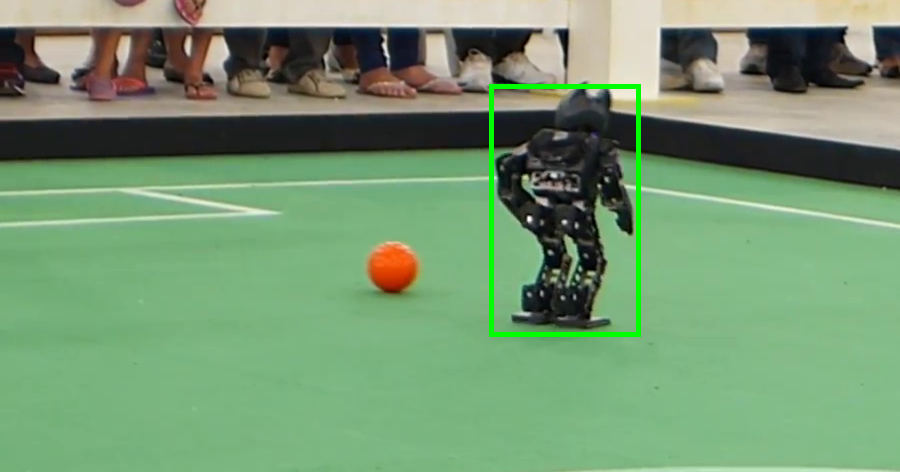
\includegraphics[width=10cm]{Imagens/HeartsHAAR.png} }}%
\caption*{Fonte: Quadro extraído do vídeo de qualificação do time Bold Hearts \cite{Bold} disponível em \citefloat{BoldHearts}.}
    \label{fig_He}%
\end{figure}

\begin{figure}[!h!t!]
\centering \caption{Curvas ROC. A linha verde mostra o algoritmo HOG-SVM clássico treinado com imagens de robôs usado para detecção de robôs.
A linha vermelha demonstra o resultado do classificador HAAR-AdaBoost treinado com o mesmo propósito.}
\includegraphics[width=12cm]{Imagens/ROCHH.png}\\
\DeclareGraphicsExtensions.
\caption*{Fonte: Autor.}
\label{fig_rocHH}
\end{figure}

As duas curvas ROC apresentadas na figura ~\ref{fig_rocHH} sugerem que os classificadores treinados parecem ser equivalentes. Devido à diversidade de robôs ambos os classificadores demonstraram capacidade de generalização que pode reconhecer diversos tipos de robôs dadas imagens de treinamento normalizadas suficientes.

Outro parâmetro de desempenho utilizado foi o de resposta dos algoritmos em quadros por segundo. É vital para um robô jogador de futebol que consiga detectar outros robôs em tempo real. A comparação desses parâmetros de desempenho estão na figura ~\ref{fig_fps}, esta informação é particularmente vital quando se trata de um robô que precisa agir rapidamente.

\begin{figure}[!h!t!]
\centering \caption{Desempenho dos descritores HAAR-AdaBoost e HOG-SVM em termos de quadros por segundo após processamento.}
\includegraphics[width=12cm]{Imagens/FPS.png}
\DeclareGraphicsExtensions.
\caption*{Fonte: Autor}
\label{fig_fps}
\end{figure}

Os resultados mostram alguma vantagem para o HAAR-Adaboost em quadros por segundo, que pôde ser utilizado em full-hd 1920x1080 pixels mas, com alguns falso positivos, já que é uma técnica sensível à mudanças de iluminação. Já o HOG-SVM foi mais preciso em termos de detecção, porém com a limitação da taxa de velocidade e por consequência a resolução máxima de 640x480 pixels. Nas figuras ~\ref{fig:Mix1} e ~\ref{fig:Mix2} as mesmas imagens demonstrando as detecções para os dois algoritmos. Nessas figuras as detecções mostraram alguma vantagem para o HOG, que demonstrou mais estabilidade detectando menos falso positivos.

Aqui cabe uma ressalva, quando se trata de avaliar os descritores, os parâmetros escolhidos e o hardware foram verdadeiramente responsáveis pelo desempenho geral dos dois algoritmos.

O tempo gasto no treinamento e na normalização e redimensionamento das imagens também foi uma questão complicada. Enquanto o HOG-SVM determinava todas as características por si só e levava no máximo 2 horas para efetuar o treinamento, o HAAR-Adaboost precisava que uma pessoa determinasse onde os objetos estavam em cada imagem positiva e seu treinamento levou de 5 a 12 horas para ser concluído. É válido lembrar que as imagens positivas do HOG-SVM precisaram ser redimensionadas o que levou um tempo considerável.


\begin{figure}[!h!t!]%
    \centering  \caption{Vários robôs identificados usando o HOG-SVM e o HAAR-AdaBoost.}%
    \subfloat[HOG - SVM]{{\includegraphics[width=15cm]{Imagens/MixHOG.png} }}%3.65
    \qquad
    \subfloat[HAAR - Boosting]{{\includegraphics[width=15cm]{Imagens/MixHAAR.png} }}%
\caption*{Fonte: Quadro extraído do vídeo de qualificação do time Bold Hearts \cite{Bold} disponível em \citefloat{BoldHearts}.}
    \label{fig:Mix1}%
\end{figure}

\begin{figure}[!h!t!]%
    \centering  \caption{Quadro de captura do robô B2 identificando vários robôs usando o HOG-SVM (Figura a) e o HAAR-AdaBoost (Figura b).}%
    \subfloat[HOG - SVM]{{\includegraphics[width=15cm]{Imagens/CIT01HOG.png} }}%3.65
    \qquad
    \subfloat[HAAR - Boosting]{{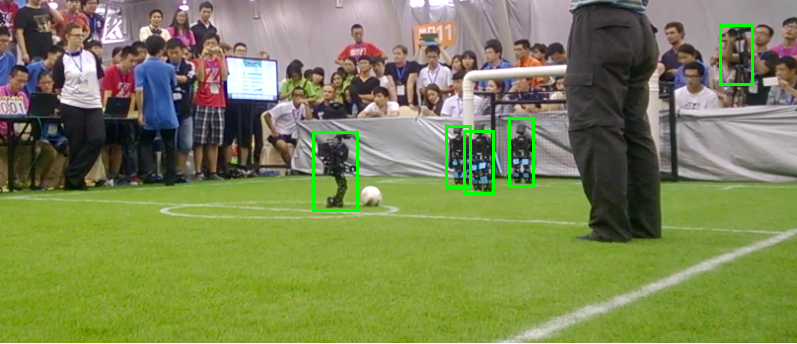
\includegraphics[width=15cm]{Imagens/CIT01HAAR.png} }}%
\caption*{Fonte: Autor.}
    \label{fig:Mix2}%
\end{figure}

\pagebreak




